% This is samplepaper.tex, a sample chapter demonstrating the
% LLNCS macro package for Springer Computer Science proceedings;
% Version 2.20 of 2017/10/04
%
\documentclass[runningheads]{llncs}
%
\usepackage{graphicx}
\usepackage{amsmath}
\usepackage{longtable}
\usepackage{float} % For precise float placement
\usepackage{subcaption} % For subtables
\usepackage{afterpage} % For forcing table to appear after current page
\usepackage{setspace} % For adjusting line spacing
% Used for displaying a sample figure. If possible, figure files should
% be included in EPS format.
%
% If you use the hyperref package, please uncomment the following line
% to display URLs in blue roman font according to Springer's eBook style:
% \renewcommand\UrlFont{\color{blue}\rmfamily}

\begin{document}
%
\title{Conversational Task Agent}
%
%\titlerunning{Abbreviated paper title}
% If the paper title is too long for the running head, you can set
% an abbreviated paper title here
%
\author{Guilherme Fernandes\inst{1}\orcidID{60045} \and
Ricardo Silva\inst{1}\orcidID{60559} \and
Vladyslav Mikytiv\inst{1}\orcidID{60735}}
%
\authorrunning{Guilherme, Ricardo, Vladyslav}
% First names are abbreviated in the running head.
% If there are more than two authors, 'et al.' is used.
%
\institute{NOVA School Of Science and Technology}
%
\maketitle              % typeset the header of the contribution
%
\begin{abstract}
Our project focuses on creating an adaptive taskbot tailored specifically for guiding users through cooking tasks. This taskbot will utilize artificial intelligence and natural language processing to interact with users, understanding their progress and constraints in real-time. The taskbot will dynamically adjust instructions based on the ingredients and cooking tools available to the user. In instances where users encounter obstacles, such as running out of ingredients or lacking specific utensils, the taskbot will intelligently adapt the recipe, offering alternative ingredient substitutions or equipment alternatives to ensure successful completion of the dish. By providing personalised guidance our taskbot aims to enhance the culinary experience.

\keywords{Taskbot  \and Word embedding \and Natural Language Processing}
\end{abstract}
%
%
%
\section{Introduction}
In recent years, word embedding has emerged as a cornerstone technology in the field of artificial intelligence, revolutionising natural language processing (NLP) tasks. This transformative approach to representing words as dense vectors in continuous vector spaces has garnered significant attention and acclaim within the AI community. The rise of word embedding has been marked by its progression from conventional methods to the creation of sophisticated models capable of capturing intricate semantic connections among words.

The inception of word embedding can be traced back to the early 2000s when researchers began exploring methods to overcome the limitations of traditional vector space models, such as bag-of-words and one-hot encoding. These initial efforts paved the way for more advanced approaches that would later reshape the field of natural language processing (NLP).

However, it wasn't until the introduction of groundbreaking techniques like Word2Vec by Mikolov et al. in 2013 and GloVe (Global Vectors for Word Representation) by Pennington et al. in 2014 that word embedding started to gain widespread attention and adoption. These models introduced novel methodologies for learning distributed representations of words based on large corpora of text, capturing intricate semantic nuances and relationships.

The allure of word embedding lies in its ability to encode semantic meaning into dense vector representations, enabling machines to understand language in a more nuanced and contextually rich manner.

The project aims to utilize embedding algorithms and large language models to develop a dialog manager between users and the taskbot. This manager will execute user requests and guide them through processes, particularly in cooking recipes, with adaptability. Leveraging a dataset containing recipes data, including ingredients, procedural steps, and difficulty levels, we utilize OpenSearch indexing to efficiently retrieve information for user queries.


\section{Algorithms and Implementation}
\subsection{Indexing}
We must implement a search index of complex manual tasks in order to allow our system to retrieve relevant information about the tasks.

\begin{figure}[!htbp]
    \center
    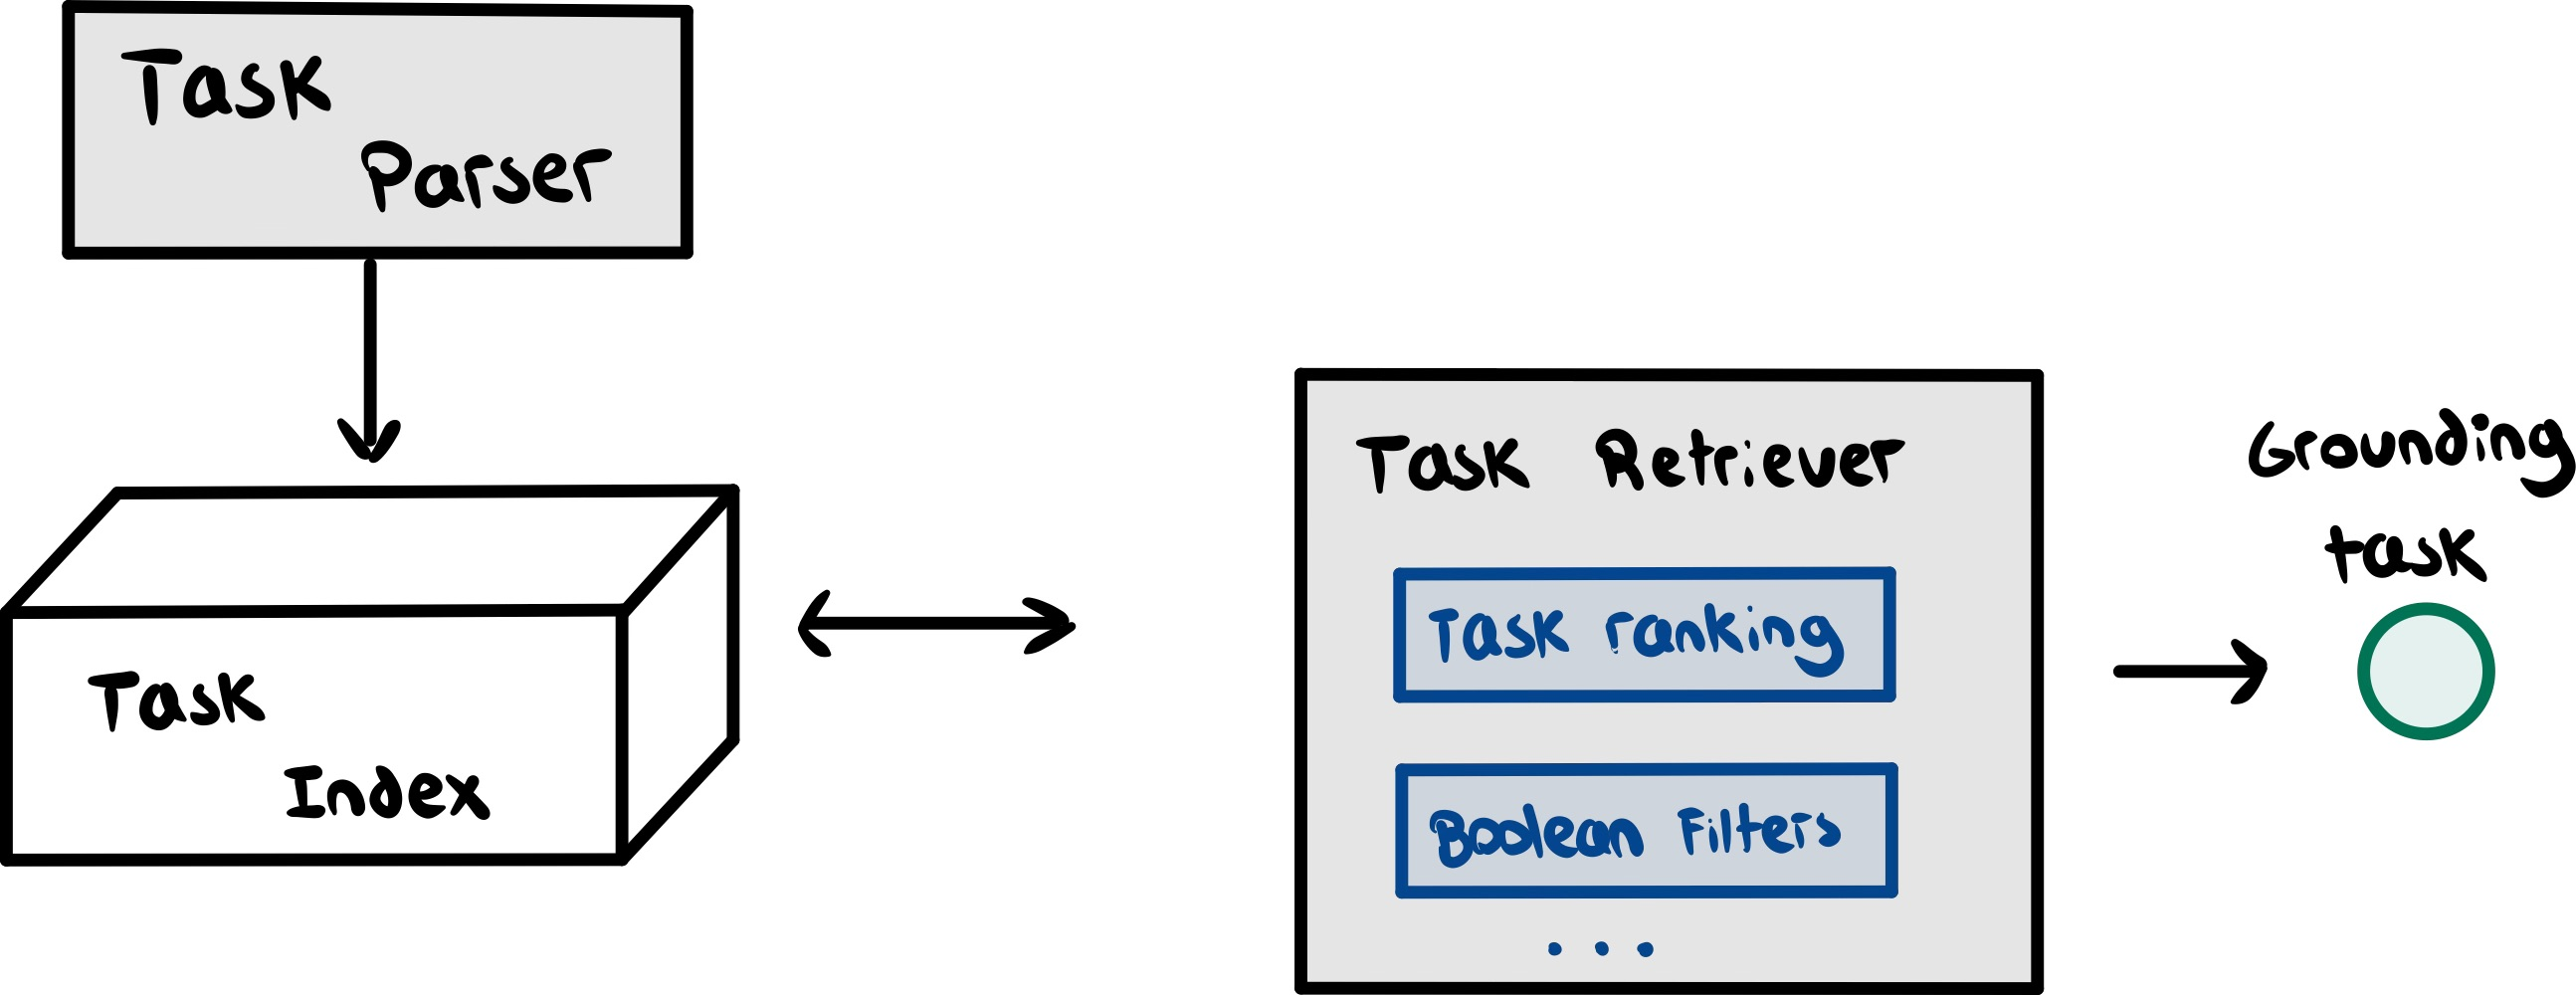
\includegraphics[scale=0.08]{images/task_retriever.jpg}
    \caption{Task retrieval}
\end{figure}

We must parse the data from the dataset which is a JSON file. We do that while we populate our indexes in OpenSearch. For each recipe we parse the JSON and send the relevant information to the index mapping that was created. We introduce a set of mappings tailored to effectively index recipe data and they are the following:

    
\begin{table}[ht]
\centering
\setlength{\abovecaptionskip}{10pt} % Adjust the spacing here
\resizebox{0.7\textwidth}{!}{%
\begin{subtable}{0.45\linewidth}
\centering
\begin{tabular}{|c|c|}
\hline
\textbf{Field} & \textbf{Data Type} \\ \hline
recipeJson & object \\ \hline
recipeName & text \\ \hline
prepTimeMinutes & integer \\ \hline
cookTimeMinutes & integer \\ \hline
totalTimeMinutes & integer \\ \hline
difficultyLevel & keyword \\ \hline
images & array of text \\ \hline
servings & float \\ \hline
\end{tabular}
\end{subtable}
\hfill % Add horizontal space between subtables
\begin{subtable}{0.45\linewidth}
\centering
\begin{tabular}{|c|c|}
\hline
\textbf{Field} & \textbf{Data Type} \\ \hline
videos & array of object \\ \hline
tools & array of text \\ \hline
cuisines & array of text \\ \hline
courses & array of text \\ \hline
diets & array of text \\ \hline
ingredients & array of object \\ \hline
stepsEmbedding & knn\_vector \\ \hline
\end{tabular}
\end{subtable}
}
\caption{Index Mapping}
\label{tab:mappings}
\end{table}

An important detail to emphasise is that our \textbf{ingredients} are a \textbf{nested type} with the properties \textbf{name} and most importantly the
corresponding \textbf{\text{ingredient\_embedding}}. We also used the mpnet-base-v2 transformer because it had better results.~\cite{mpnet}.

\subsection{Searching}
We've initiated the project by focusing on leveraging indexes for efficient dataset navigation, and OpenSearch emerges as a pivotal tool for executing queries seamlessly.

We've commenced with text-based queries, enabling users to access recipes based on various parameters such as cooking time, difficulty level, course type, or serving size.

Moreover, the integration of boolean queries adds another layer of flexibility, empowering users to refine their searches by specifying ingredients they desire or wish to avoid in their recipes.

Embedded queries stand out as particularly intriguing among our query types. By transforming user inputs into vector representations, we can uncover recipes closely related to the query. This method offers personalised recipe recommendations that align with users' interests more effectively.

In our index mappings, we utilize various embeddings to facilitate our searches. A crucial component is a model, referenced as~\cite{bert}, which extracts relevant information from natural language phrases, particularly focusing on ingredient extraction from user queries. This model also aids in processing the textual content within recipe steps.

Acknowledging the significance of recipe steps, we've introduced embeddings for both the recipe names and their corresponding individual steps. This approach enables our search system to capture the essence of each recipe efficiently, ensuring accurate query results.

After thorough testing, we've identified the most effective embeddings for our system: ingredient embeddings for individual ingredients and step embeddings paired with respective recipe names. Despite transformer limitations, these embeddings show promising results, especially in user-input based embedded queries. Given that our system doesn't prioritize contextual nuances in phrases, we've opted to utilize FoodBERT~\cite{bert} to maintain consistency with this approach.

In essence, our framework enables a dynamic exploration of the dataset, granting users the ability to refine their searches precisely according to their preferences and specific requirements.

\section{Evaluation}
\subsection{Dataset Description}
The dataset contains a significant amount of recipe information, but not all of it is pertinent to our objectives. After careful examination, we have identified the essential data required for generating meaningful embeddings and providing accurate search results to users. Our focus has been on excluding irrelevant information and prioritizing specific details that enhance the user's search experience.

Following a thorough dataset analysis, we selectively filtered the essential data required for crafting our embeddings and information pertinent to users for search results. Our assessment highlighted the necessity for detailed information on certain aspects while deeming others less crucial.

During our process of embedding sentences and experimenting with various techniques, we encountered two significant problems. Firstly, the \textbf{displayText} of each ingredient contained excessive information, including opinions and irrelevant text. Secondly, some \textbf{displayText} entries were in languages other than English (e.g., Italian). This posed challenges, as searching for ingredients like Italian cheese would erroneously suggest a strong relationship due to language inconsistencies.

Therefore, to address these issues, we implemented two solutions. Firstly, we opted to utilize only the \textbf{ingredient} property of each ingredient. To accomplish this, we employed a model that extracts the ingredient from the \textbf{displayText} and populates the ingredient field in the JSON.

For that, we used the \url{https://github.com/strangetom/ingredient-parser}~\cite{ingredientParser} in order to extract the ingredients from a phrase. With this we solved the issue of having \textbf{null} values in these fields. However, the problem persisted with \textbf{textDisplay} being in another language, as the ingredient parser model~\cite{ingredientParser} simply returned the \textbf{displayText} as it was originally.

By utilizing a translator model~\cite{deeptranslate} before feeding the data to the ingredient parser~\cite{ingredientParser}, we successfully translated the \textbf{displayTexts} that were in other languages into English. This allowed us to apply the model to extract the ingredients and populate the missing fields.

These modifications to our original dataset resulted in a more comprehensive dataset. We created a new JSON file containing all of the original information along with the additional data. This file is accessible through OpenSearch, as it is stored without being indexed. Its sole purpose is to be retrievable from OpenSearch.

\bibliographystyle{plain}
\bibliography{my_bib.bib}

\end{document}
